\chapter{Advanced topics}

\section{Sequences of functions}

\begin{definition}[Power series]
    A power series about $x_0$ is series of the form:
    \begin{equation*}
        \sum \limits_{n = 0}^\infty a_n(x - x_0)^n
    \end{equation*}
\end{definition}

\begin{theorem}
    Suppose $\{|a_n|^{1/n}\}$ converges, \emph{i.e.}:
    \begin{equation*}
        R = \lim \limits_{n \to \infty} |a_n|^{n/n}
    \end{equation*}
    and define $p$, the \emph{radius of convergence}, as:
    \begin{equation*}
        p = \begin{cases}
            \frac{1}{R} \text{ if } R > 0 \\
            \infty \text{ if } R = 0
        \end{cases}
    \end{equation*}
    Then:
    \begin{enumerate}
        \item If $|x-x_0| < p$, the series $\sum a_n(x - x_0)^n$ converges;
        \item If $|x-x_0| > p$, the series diverges.
    \end{enumerate}
\end{theorem}

\begin{proof}
    First, notice that:
    \begin{equation*}
        \lim \limits_{n \to \infty} |a_n(x-x_0)^n|^{1/n} = R |x-x_0|
    \end{equation*}
    So, the theorem is valid from the Root test.
\end{proof}

Suppose $\sum a_n(x-x_0)^n$ is a power series with radius of convergence $p$. Then, define $f: (x_0 - p, x_0 + p) \to \R$ such that:
\begin{equation*}
    f(x) := \sum \limits_{n=0}^\infty a_n (x - x_0)^n
\end{equation*}

So, $f(x)$ is a limit of a sequence of functions $f_n(x)$, \emph{i.e.}:

\begin{equation*}
    f(x) = \lim \limits_{m \to \infty} f_m(x)
\end{equation*}

Where,

\begin{equation*}
    f_m(x) = \sum \limits_{n=0}^m a_n(x-x_0)^n
\end{equation*}

The definition of a function in such form leads to a number of questions:
\begin{enumerate}
    \item Is $f(x)$ continuous?
    \item Is $f(x)$ differentiable, and does $f'(x) = \lim_{n \to \infty} f'_m(x)$?
    \item If $f(x)$ is continuous, does it mean:
        \begin{equation*}
            \int_a^b f(x) \dint x = \lim \limits_{n \to \infty} \int_a^b f_m(x) \dint x \text{ ?}
        \end{equation*}
\end{enumerate}

In order to answer these questions, some tools must be build first.

\subsection{Pointwise and uniform convergence}

We start from framework more general than power series.

\begin{definition}[Pointwise convergence]
    Define $f:S \to \R$ and $f_n: S \to \R$ with $n \in \N$. The sequence of functions $\{f_n\}$ is said to convergence pointwise to $f$ if:
    \begin{equation*}
        \lim \limits_{n \to \infty} f_n(x) = f(x), \forall x \in S
    \end{equation*}
\end{definition}

\paragraph{Examples}

\begin{enumerate}
    \item Consider $f_n(x) = x^n$ on $[0,1]$. Then,
        \begin{equation*}
            \lim \limits_{n \to \infty} f_n(x) = \begin{cases}
                0 \text{ if } x \in [0,1) \\
                1 \text{ if } x=1
            \end{cases}
        \end{equation*}
        Thus $\{f_n(x)\}$ converges pointwise to the function above, hence a sequence of continuous function may not converge to a continuous function.
    \item Consider $f_n(x) = \sum_{m=0}^n x^m$ for $x \in (-1,1)$. Then,
        \begin{equation*}
            \lim \limits_{n \to \infty} f_n(x) = \lim \limits_{n \to \infty} \sum \limits_{m=0}^n x_m = \frac{1}{1-x}
        \end{equation*}
\end{enumerate}

\begin{figure}[H]
    \centering
    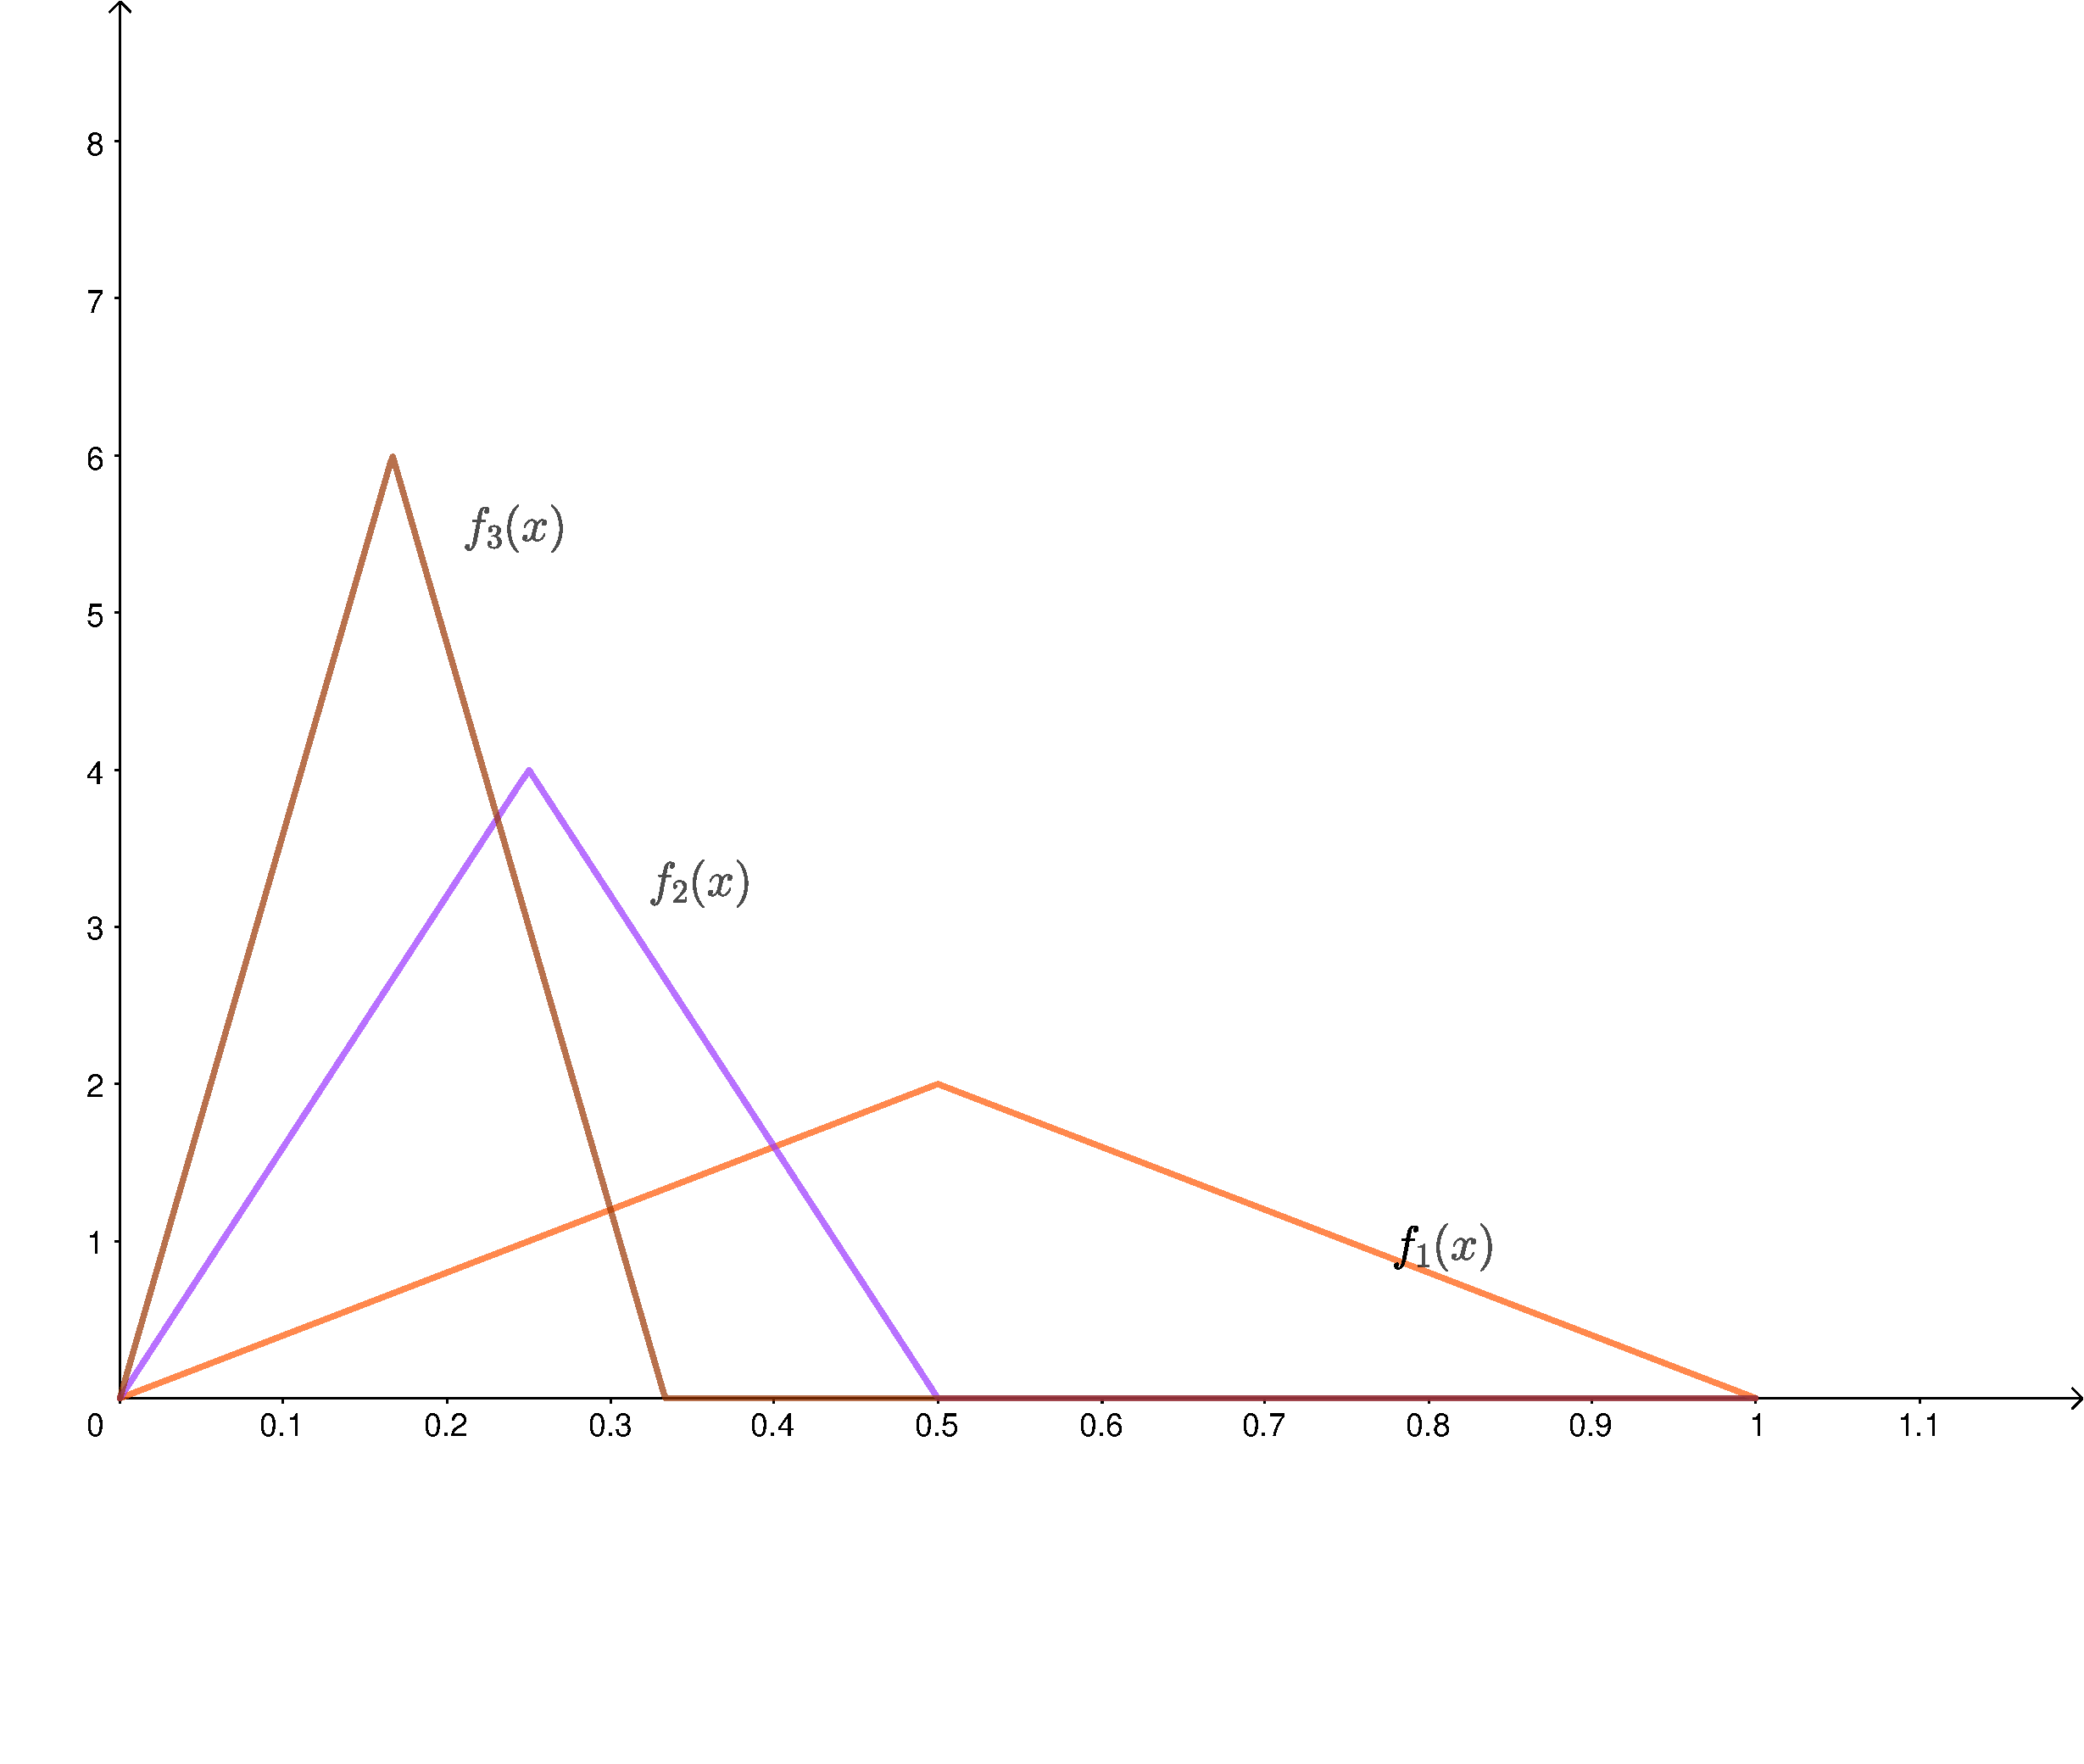
\includegraphics[width=0.75\textwidth]{images/06_sequence_functions.pdf}
    \centering
\end{figure}